% main.tex -- parent TeX file
\documentclass[a4paper,uplatex]{jsreport}

%画像の設定
\usepackage[dvipdfmx]{graphicx} %画像を貼る
\usepackage{float} %画像の位置
\usepackage{here}


\usepackage[dvipdfmx]{hyperref} %リンクとその設定
\usepackage{pxjahyper}
\hypersetup{setpagesize=false, bookmarksnumbered=true, bookmarksopen=true, colorlinks=false, linkcolor=black, citecolor=black, }

%便利なコマンド
\usepackage{url} %URLコマンド\usl
\usepackage{siunitx} %SI単位コマンド\si
\usepackage[version=3]{mhchem} %化学式コマンドce
\usepackage{bm} %ベクトル太字

\usepackage{biblatex}
\addbibresource{reference.bib}

\begin{document}

\title{宇宙線ミューオンが起こす光生成反応の探索}
\author{1843105s 安 博充\\
        1863121s 山下 智愛\\
        1823185s 濱田 悠斗
}
\date{\today} %date \today or 2100/01/01

\maketitle %タイトル
\tableofcontents %目次
%\listoffigures %図目次
%\listoftables %表目次

%アブスト
aaagtgtgt
優しいね
test hamada

%本文
\chapter{目的} \label{cha:introduction}

\section{目的}
あああ
\chapter{散乱断面積の計算} \label{cha:cross_section}
計算するための仮定や使用する式について説明し散乱断面積を導出し、予定する検出器でのイベント数の見積もりを行う。

\section{散乱断面積の計算に用いる仮定}
\subsection{ハドロン系の質量の仮定}
2粒子以上の多粒子状態に崩壊する場合、ハドロン中間状態の質量$m_W$ は バリオン数を保存し最も軽い2粒子の組み合わせである$\pi$ の質量$m_\pi$と陽子の質量 $m_p$の合計よりも大きくなければならない。

\begin{equation}
    m_W \geq m_\pi + m_p \approx 0.14 + 0.94 = 1.08 \ \mathrm{GeV}
\end{equation}
よって、ハドロン系の質量は$m_W \geq 1.08$ GeVを仮定する。

\subsection{光子のエネルギーの仮定}
図\ref{fig:sigma1}のように核子と光子の四元運動量を考える。
\begin{figure}[H]
    \centering
    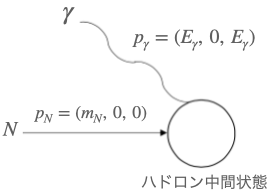
\includegraphics[height=5cm]{img/diagram_momentum.png}
    \caption{ハドロン中間状態と核子と光子の図}
    \label{fig:sigma1}
\end{figure}
核子、光子の四元運動量をそれぞれ$p_N$, $p_\gamma$とすると、
\begin{equation}
    p_N = (m_N, 0, 0),\  p_\gamma = (E_\gamma, 0,  E_\gamma)
\end{equation}
とかける。
$m_W$との関係は
\begin{equation}
    \label{eq2_2}
    m_W^2 = (p_N + p_\gamma)^2 = p_N^2 + 2p_N p_\gamma + p_\gamma^2
    = 2m_N E_\gamma + m_N^2
\end{equation}
$m_N$ = 0.94 GeVであるから、\ref{eq2_2}式を用いると$m_W$ = 1.08 GeV の時
\begin{equation}
    E_\gamma \approx 0.23 \ \mathrm{GeV}
\end{equation}
よって、光生成反応を観測するために必要な光子のエネルギー$E_\gamma$は
$E_\gamma \geq 0.23 \ \mathrm{GeV}$となる。


\subsection{宇宙線$\mu$の仮定}
宇宙線$\mu$ のエネルギー$E_\mu$ は$E_\gamma$ よりも遥かに大きいエネルギーを持つ必要がある。
そのため$E_\mu = 1.5$ GeV とおく。
また$E_\mu = 1.5$ GeV 以上となる$\mu$ の割合Rは図\ref{fig:sigma2}より$R \approx 0.56$ と頻度が高めである。
\begin{figure}[H]
    \centering
    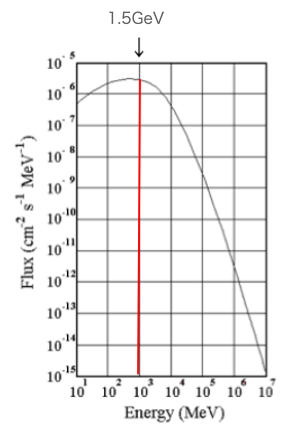
\includegraphics[height=5cm]{img/cosimic_ray_energy_distribution.png}
    \caption{宇宙線$\mu$のエネルギー分布 \cite{cosmic_ray}}
    \label{fig:sigma2}
\end{figure}
$E_\mu$と散乱後の$\mu$のエネルギー$E'_\mu$ との比をyとして、その値は
\begin{equation}
    y = \dfrac{E_\mu - E'_\mu}{E_\mu} \approx 0.2
\end{equation}
となる。

\section{生成断面積の計算枠組み}
$\mu$とNの散乱断面積$\sigma_{\mu N}$は$\mu$から$\gamma$を出す確率$\Phi$と、
$\gamma$とNとの散乱断面積$\sigma_{tot}(\gamma^* N)$の積で表すことができる。
\begin{equation}
    \sigma_{\mu N} =\int dy  \sigma_{tot}(\gamma^* N) \Phi
\end{equation}
$\Phi$は以下のように表される。
\begin{equation}
    \Phi(y) = \dfrac{\alpha}{\pi y} \int \dfrac{dQ^2}{Q^2} [(1-y)(1 - \dfrac{Q^2_{min}}{Q^2}) + \dfrac{y^2}{2}]
\end{equation}
$Q^2 = - (k - k')^2 $を運動量移行の2乗の負数とした。

\section{\texorpdfstring{$\Phi$}{LG}の考察}\label{section2_3}
$\Phi$の積分前の値はyを定数とすると図\ref{fig:sigma3}のようになる。
\begin{figure}[H]
    \centering
    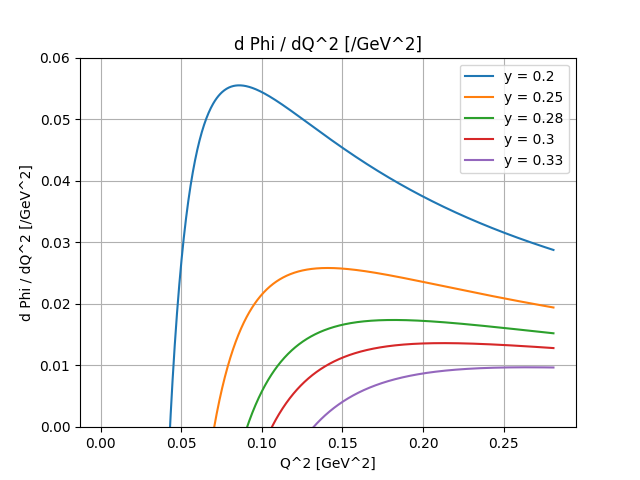
\includegraphics[height=7cm]{img/flux_fixed_y.png}
    \caption{$\dfrac{d\Phi ^2}{dydQ^2}$ のyを定数としたグラフ}
    \label{fig:sigma3}
\end{figure}
このグラフから$\Phi$はyが小さいところで大きくなる。つまり、$E_\mu$ が $E_\gamma$より遥かに大きくなるところで$\sigma_{\mu N}$が大きくなる。
また、$Q^2$が小さくなるところで大きくなっている。$Q^2$は0でない最小値を持つ。この最小値を$Q^2_{\mathrm{min}}(y)$とすると、以下のように表される。
\begin{equation}
    \label{eq2_8}
    Q^2_{\mathrm{min}} = \dfrac{m_p^2 y^2}{1-y}
\end{equation}

\section{断面積の計算に用いる近似}
\ref{section2_3}章で示したように断面積を概算するには y が小さいところを見積もればよいことがわかる。
宇宙線ミューオンのエネルギーを 1.5 GeV としたことから、
$0.2 < \mathrm{y} < 0.33$ に対応する $E_\gamma \in [300, 500]$ MeV の範囲の断面積を見積もる。
図\ref{fig:sigma4}は核子1個あたりの全光核反応断面積と光子のエネルギーの関係であり、これを用いて$\gamma$とNの反応断面積$\sigma_{tot}(\gamma^* N)$を
$\sigma_{tot}(\gamma^* N) = 0.3$ mbと近似する。
\begin{figure}[H]
    \centering
    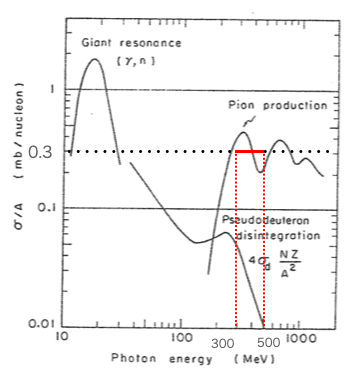
\includegraphics[height=7cm]{img/sigma_tot.png}
    \caption{核子1個あたりの全光核反応断面積と光子のエネルギーの関係}
    \label{fig:sigma4}
\end{figure}
$E_\mu = 1.5 \mathrm{GeV}$,$E_\gamma \in [0.3, 0.5] \mathrm{GeV}$の仮定からyの範囲は
\begin{equation}
    y = \dfrac{E_\gamma}{E_\mu}
\end{equation}
を用いることで$y \in [0.20, 0.33]$となる。

\section{\texorpdfstring{$yとQ^2$}{LG}の積分範囲}
$m_W$の関係式
\begin{equation}
    m_W = \sqrt{m_p^2 + 2m_pE_\mu y - Q^2}
\end{equation}
は
$m_W = 1.08$GeVとした時、図\ref{fig:sigma5}のようになる。
\begin{figure}[H]
    \centering
    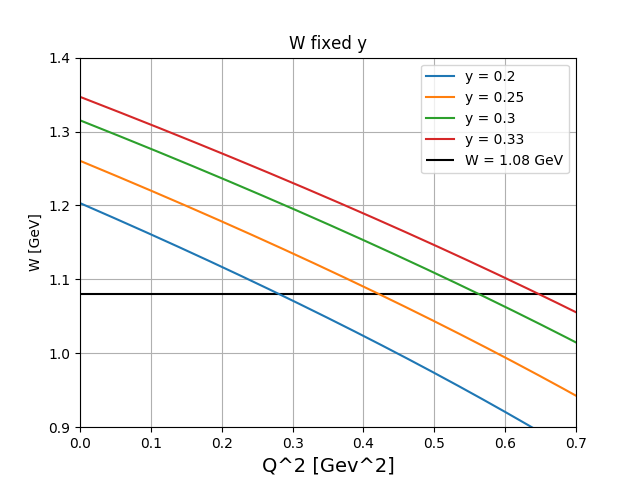
\includegraphics[height=7cm]{img/W2_fixed_y.png}
    \caption{$m_W = \sqrt{m_p^2 + 2m_pE_\mu y - Q^2}$のyを固定した関係式}
    \label{fig:sigma5}
\end{figure}
$m_W = 1.08$GeVの直線とyの値ごとの直線が交わる$Q^2$の値が$Q^2$の最大値になるのでこれを$Q^2_{\mathrm{max}}$とする。
よって、積分範囲は$y \in [0.20, 0.33], Q^2 \in [Q^2_{\mathrm{min}}(y), Q^2_{\mathrm{max}}(y)]$となる。

\section{断面積の計算}
$\dfrac{d^2\sigma}{dydQ^2}$は図\ref{fig:sigma6}のようになる。
\begin{figure}[H]
    \centering
    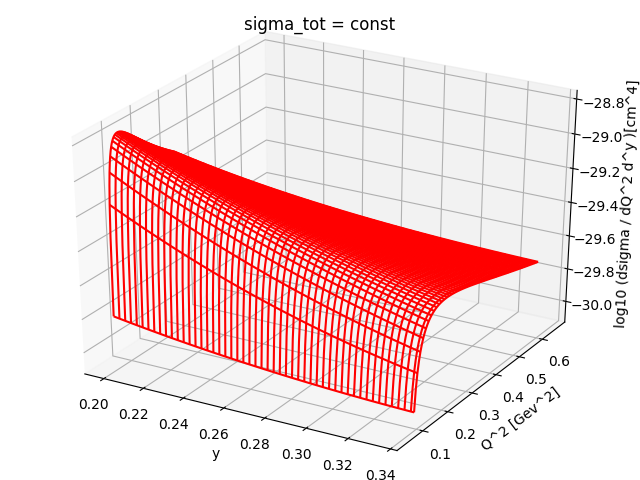
\includegraphics[width=8cm]{img/integrate_flux_used_artile.png}
    \caption{$\dfrac{d^2\sigma}{dydQ^2}$の3次元プロット}
    \label{fig:sigma6}
\end{figure}
これを積分すると、断面積$\sigma$は、$\sigma \approx 3.3 \times 10^{-28} \ \mathrm{cm^2}$となった。

\section{予定する検出器でのイベント数の見積もり}
関係式
\begin{equation}
    -dN =\dfrac{\rho N_A \sigma }{A}NRV
\end{equation}
から反応式を見積もる。
$-dN$を入射$\mu$の単位時間あたりの減少分、検出器の密度$\rho = 1.0 \ \mathrm{g/cm^2}$、
検出器の質量数$A = 12 \ \mathrm{g/mol}$、検出器の有効体積$V = 7500 \ \mathrm{cm^3}$、
単位時間・単位面積あたりの入射する$\mu$の数を$N = \dfrac{1}{10\times 10} \ \mathrm{個/s\cdot cm^2}$、
1.5GeV以上のエネルギーを持つ$\mu$の割合を$R = 0.56$として代入すると
\begin{equation}
    -dN \approx 4.4 \times 10^{-4} \ \mathrm{個/s}
\end{equation}
となった。
このことから反応するイベントは$10^4$オーダーに1個であることがわかる。

実際の実験での反応数の見積もりは、\ref{sec:anal:data}節で述べる。
\chapter{散乱角度}\label{cha:angle}
\section{光生成反応の散乱角度}
図\ref{fig:angle1}のように実験室系での$\mu$の散乱角$\theta$,中間状態$\gamma^*N$系の散乱角$\phi$を定義する。
\begin{figure}[H]
    \centering
    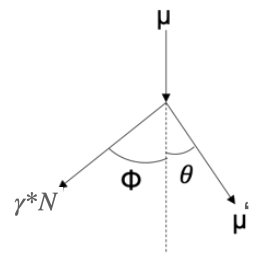
\includegraphics[height=4cm]{img/angle_diagram.png}
    \caption{散乱角$\theta, \phi$の定義}
    \label{fig:angle1}
\end{figure}

\subsection{$\theta$の取る値}
図\ref{fig:angle2}のような運動学変数を考える。
\begin{figure}[H]
    \centering
    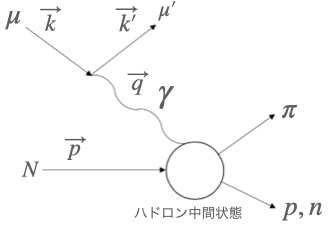
\includegraphics[height=4cm]{img/diagram_3momentum.png}
    \caption{運動学変数の定義}
    \label{fig:angle2}
\end{figure}
各値に対して以下のような定義を行う。
このとき、$\mu$の進行方向の運動量成分を
$p_\parallel$, 垂直方向の成分を $p_\perp$ として、4元運動量を
$p = (E, p_\parallel, p_\perp) $とあらわすと、各粒子の運動量は以下の通りとなる。
\begin{equation}
    k = (E_\mu , p_\mu,0)
\end{equation}
\begin{equation}
    k' = (E'_\mu, p'_\mu \cos\theta, p'_\mu \sin\theta)
\end{equation}
\begin{equation}
    p = (m_N, 0, 0)
\end{equation}
\begin{equation}
    q = k-k'=(E_\mu - E'_\mu, p_\mu-p'_\mu \cos\theta, -p'_\mu \sin\theta)
\end{equation}
また、$Q^2$は$q$を用いることにより式\ref{eq3_1}のように表せる。
\begin{equation}
    \label{eq3_1}
    Q^2 = -q^2 = 2E_\mu E'_\mu -2m^2_\mu-2p_\mu p'_\mu \cos\theta
\end{equation}
式\ref{eq3_1}を$\theta$について解く。

$E'_\mu = E_\mu(1-y), p'_\mu = \sqrt{E'^2_\mu - m^2_\mu}$
を用いて$E'_\mu, p'_\mu$を消去すると、
\begin{eqnarray}
    \theta & = &\arccos \left( \dfrac {2E_\mu E'_\mu -2m^2_\mu-Q^2}{2p_\mu p'_\mu} \right) \\
    & = & \arccos \left(\dfrac{-Q^2-2m^2_\mu+2E^2_\mu(1-y)}{2\sqrt{E^2_\mu-p^2_\mu}\sqrt{E^2_\mu(1-y)^2-m^2_\mu} }  \right)
\end{eqnarray}
この$\theta$は図\ref{fig:angle3}のようになる。
\begin{figure}[H]
    \centering
    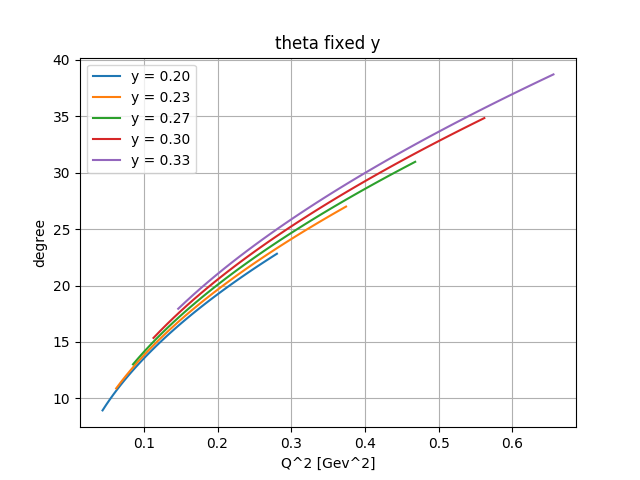
\includegraphics[height=5cm]{img/theta_degree_y_fixed.png}
    \caption{$\mu$の散乱角$\theta$の$Q^2$依存性}
    \label{fig:angle3}
\end{figure}
$\theta$はyが小さくなると小さくなる。また$Q^2$が小さくなると小さくなる。
$\theta$は$\theta=[10^\circ,40^\circ]$の範囲であることがわかる。

\subsection{$\phi$の取る値}
\begin{equation}
    \vec{p_\mu} \cdot \vec{p_W} = |p_\mu| |p_W| \\ \cos\phi
\end{equation}
から
\begin{equation}
    \phi = \arccos \left( \dfrac{yE^2_\mu + \dfrac{Q^2}{2}} {\sqrt{(E^2_\mu - m^2_\mu)(y^2E^2_\mu+Q^2)}} \right)
\end{equation}
$\phi$は図\ref{fig:angle4}のようになる。
\begin{figure}[H]
    \centering
    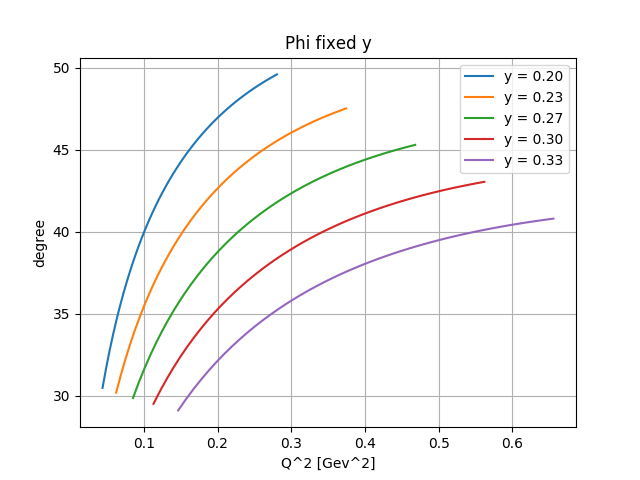
\includegraphics[width=8cm]{img/Phi_degree_fixed_y.png}
    \caption{中間状態の散乱角$\phi$の$Q^2$依存性}
    \label{fig:angle4}
\end{figure}
中間状態の散乱角$\phi$はyが小さくなると大きくなる。また、$Q^2$が小さくなると小さくなる。
$\phi$は$\phi = [30^\circ, 50^\circ]$ の範囲にあることがわかる。

\section{\texorpdfstring{$\gamma N$の崩壊で生成される$\pi, p$について}{LG}}
\subsection{$\gamma^* N$から生成される$\pi,p$の静止系での運動量とエネルギー}
\begin{figure}[H]
    \centering
    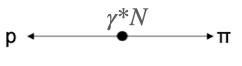
\includegraphics[width=6cm]{img/rest_middle_situation.png}
    \caption{静止した$\gamma^* N$から生成される$\pi,p$}
    \label{fig:angle5}
\end{figure}
図\ref{fig:angle5}のような静止した$\gamma^* N$を考える。
$m_W = 1.08 \ $GeV, $E_\mu = 1.5 \ $GeVを仮定する。
この仮定から$y = 0.2$で$Q^2 \approx 0.28 \ \mathrm{GeV^2}$となる。
それぞれの粒子が持つエネルギーと運動量を導出する。
エネルギー保存則から
\begin{equation}
    \label{eq3_3}
    E_W = E_\pi + E_p
\end{equation}
運動量保存則から
\begin{equation}
    \label{eq3_4}
    p_p = p_\pi
\end{equation}
式\ref{eq3_3}, \ref{eq3_4}から
\begin{eqnarray}
    E_W  & =  & E_\pi + \sqrt{m_p^2 + p_p^2} \\
    & = & E_\pi + \sqrt{m_p^2 + p_\pi^2} \\
    & = & E_\pi + \sqrt{m_p^2 + E_\pi^2 - m_\pi^2}
\end{eqnarray}
$E_\pi$について解くと
\begin{equation}
    E_\pi = \dfrac{E_W ^2 + m_\pi ^2 - m_p ^2}{2E_W}
\end{equation}
同様に$E_p$を導出すると、
\begin{equation}
    E_p = \dfrac{E_W ^2 + m_p ^2 - m_\pi ^2}{2E_W}
\end{equation}
運動量は関係式
\begin{equation}
    p^2 = \sqrt{E^2 - m^2}
\end{equation}
から見積もる。
$E_W = 1.15 \ $GeV, $m_p = 0.938 \ $GeV, $m_\pi = 0.138 \ $GeVとして代入すると、
$E_π = 200.7 \ $MeV, $E_p = 949.0 \ $ MeV , $p_π = p_p = 145.8 \ $ MeVとなる。

\subsection{実験室系にブーストされた$\gamma^* N$から生成される$\pi,p$の運動量}
\begin{figure}[H]
    \centering
    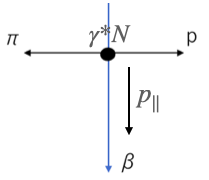
\includegraphics[height=3cm]{img/boost_middle_situation.png}
    \caption{実験室系にブーストされた$\gamma^* N$から生成される$\pi,p$}
    \label{fig:angle6}
\end{figure}
実験室系にブーストされた$\gamma^* N$を考える。
ローレンツ変換の式\ref{eq3_5}を用いて運動量を計算する。
\begin{equation}
    \label{eq3_5}
    \left(\begin{array}{c}
            E^* \\
            p^*_\parallel
        \end{array}\right)
    =\left(\begin{array}{cc}
            \gamma \ \ -\gamma \beta \\
            -\gamma \beta  \ \  \gamma
        \end{array}\right)
    \left(\begin{array}{c}
            E \\
            p_\parallel
        \end{array}\right)
\end{equation}
ここで
\begin{eqnarray}
    \beta = \dfrac{p_W}{E_W} = \dfrac{p_\gamma + p_p}{E_\gamma + E_p} = 0.24
\end{eqnarray}

\begin{eqnarray}
    \gamma = \dfrac{1}{\sqrt{1 - \beta^2}} \approx 1.03
\end{eqnarray}
となる。
このことから中間状態はあまりブーストされないことがわかる。

\begin{figure}[H]
    \centering
    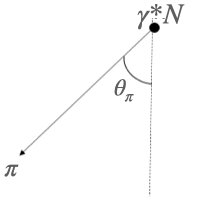
\includegraphics[height=5cm]{img/theta_pi.png}
    \caption{静止した$\gamma^* N$から出てくる$\pi$の散乱角}
    \label{fig:angle7}
\end{figure}

静止した$\gamma^* N$系から$\pi$が出てくる角を$\theta_\pi$として、
$\pi$の運動量について考える。
$\gamma^* N$系の進行方向に対して垂直な運動量成分を$p_{\pi \perp}$、平行な運動量成分を$p_{\pi \parallel}$とすると以下の式が成り立つ。

\begin{eqnarray}
    p_{\pi \parallel} = p_\pi  \cos\theta \\
    p_{\pi \perp} = p_\pi \sin\theta
\end{eqnarray}

\section{\texorpdfstring{実験室系にブーストされた$\gamma^* N$から生成される$\pi$の散乱角}{LG}}
ローレンツ変換の式から$p'_{\pi \parallel}$を導出し、$p_{\pi \perp} = p'_{\pi \perp}$であるから、
\begin{equation}
    p'_\pi = \sqrt{p'^2_{\pi \parallel} + p'^2_{\pi \perp} }
\end{equation}
$\theta_\pi$が等方的に出た時にブーストされた$\gamma^* N$から出てくる$\pi$の角度を$\phi_\pi$とすると,
\begin{equation}
    p'_{\pi \parallel} = p'_\pi \cos{\phi_\pi}
\end{equation}
よって、
\begin{equation}
    \phi = \arccos{\dfrac{p'_{\pi \parallel}}{p'_\pi}}
\end{equation}
$\theta_\pi$が等方的に出るとして$\phi_\pi$の分布は\ref{fig:angle8}のようになった。
\begin{figure}[H]
    \centering
    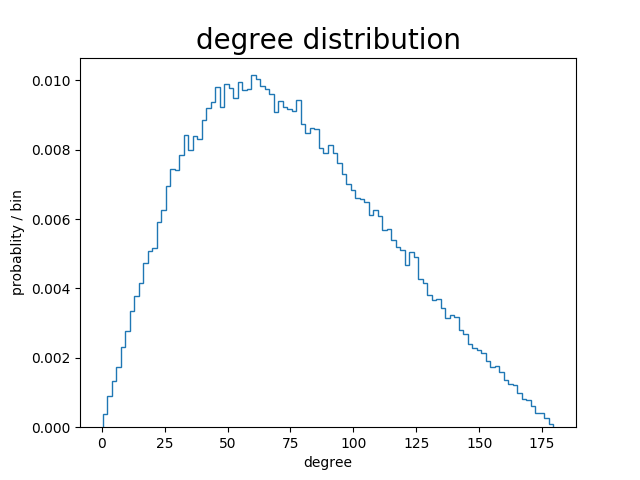
\includegraphics[height=7cm]{img/degree_distribution.png}
    \caption{$\pi$の角度分布}
    \label{fig:angle8}
\end{figure}
$\phi_\pi$は60°付近にピークを持つため主に進行方向成分が大きいが、
同時に横方向の運動量成分も大きいことがわかる。
\chapter{装置} \label{equipment}
\section{装置の概念設計}

\section{細かい設計}
\chapter{simulation}\label{simulation}
\section{Geant4}
Geant4 とは物質中を通過する粒子の物理相互作用をモンテカルロ法に基づいてシミュレートすることのできるパッケージである.
物理プロセスや検出器の構造, 検出器の応答, 応答データ等の作成, 保存などの多くのツールキットから構成されている.

\section{本実験での$\mu$粒子シミュレーション}
宇宙線発生シミュレーションCRYを用いて$\mu$粒子を生成した.
装置のパラメーターは
\begin{quote}[H]
    \begin{itemize}
        \item トリガーシンチレータ126cm$\times$7cm$\times$1cmを7度ずつ傾けて横に3枚
        \item シンチレータ75cm$\times$4cm$\times$1cmを横に4枚, 縦に8層
        \item アルミニウム板100cm$\times$30cm$\times$2cmを8層
    \end{itemize}
\end{quote}
としてトリガーシンチレータのすぐ下からトリガーシンチレータの大きさの範囲で$10^{7}$イベントの$\mu$粒子を発生させた.
\\
CRYによって生成した$\mu$粒子のうち、
1番上のシンチレータに入射した粒子のエネルギー分布と角度分布がそれぞれ図\ref{fig:muon_energy_distribution}、図\ref{fig:muon_degree_distribution}である。
\begin{figure}[H]
    \begin{minipage}[b]{0.47\linewidth}
        \centering
        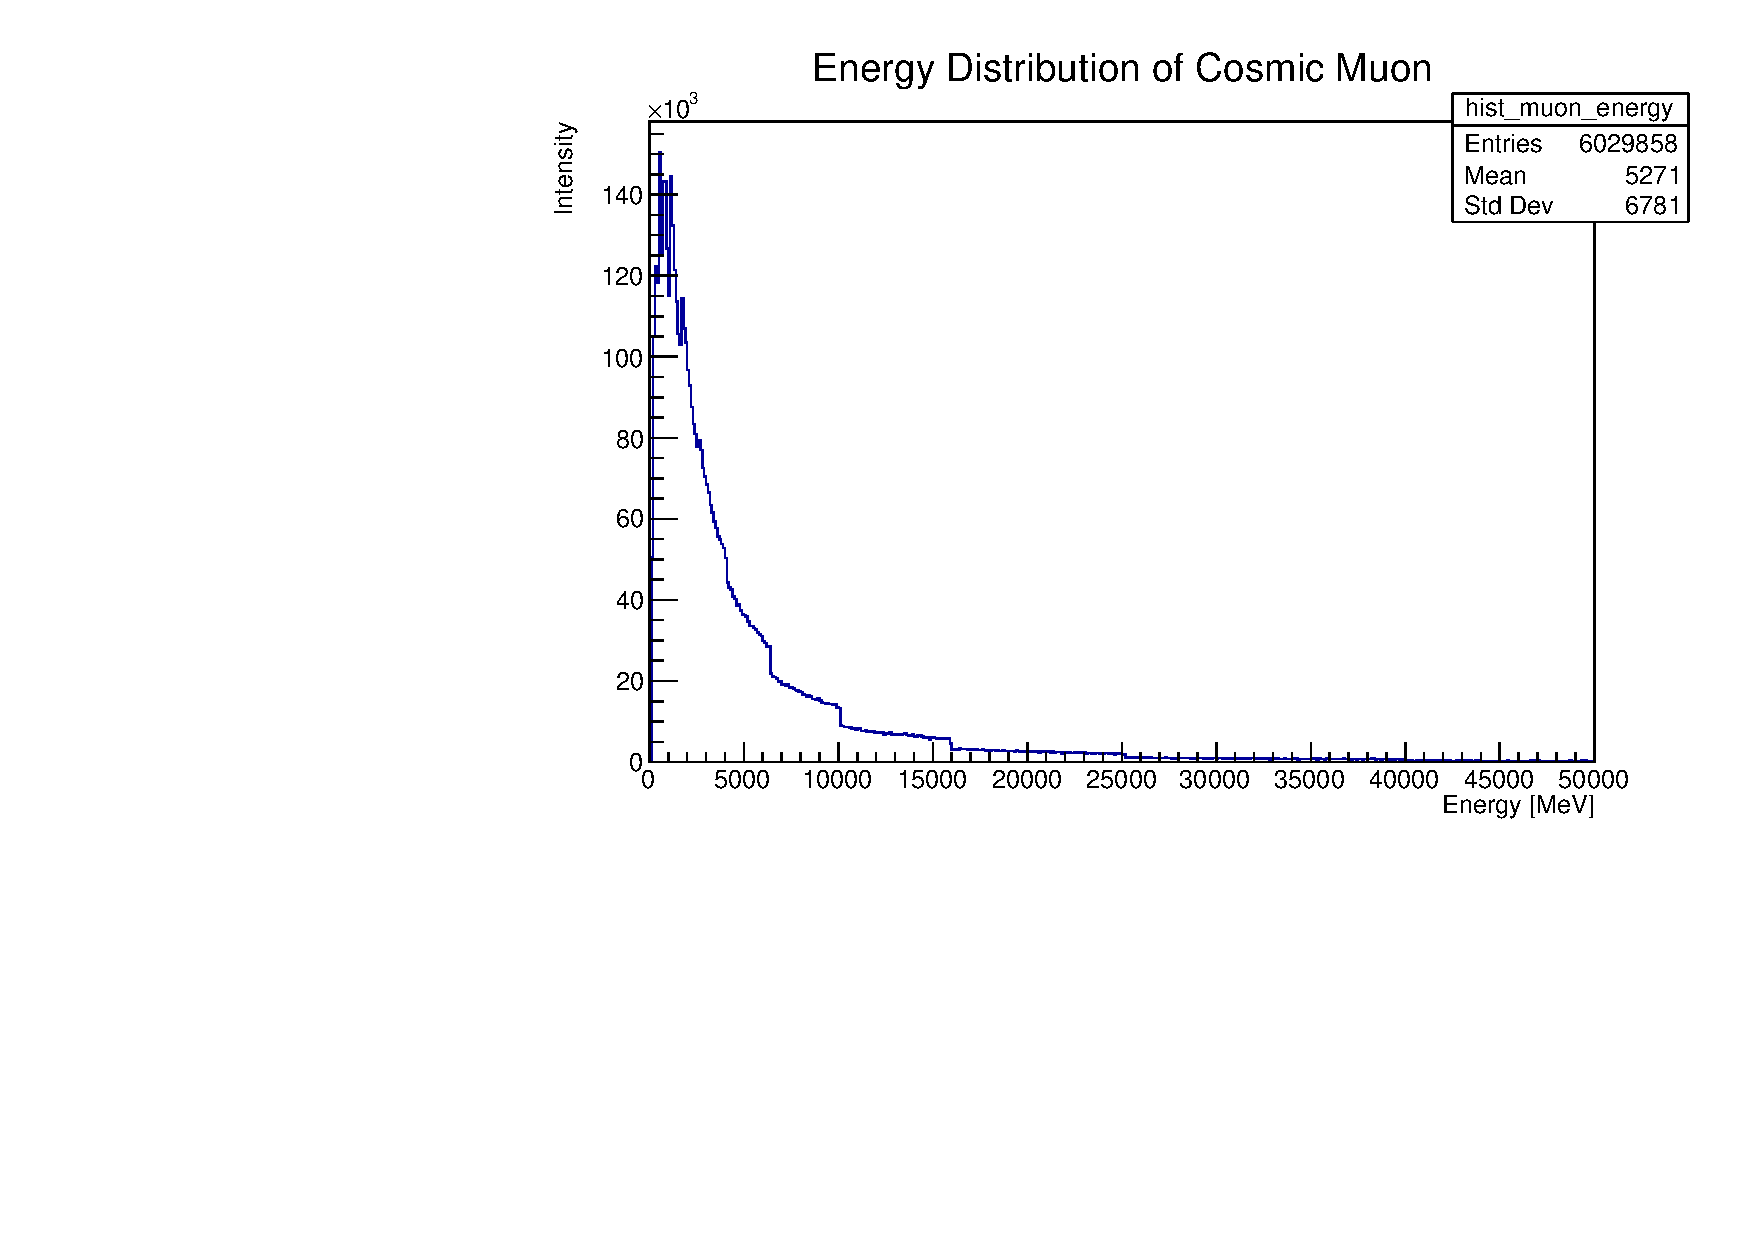
\includegraphics[height=5cm]{img/muon_energy_distribution.pdf}
        \caption{CRYによって生成した$\mu$粒子のエネルギー分布}
        \label{fig:muon_energy_distribution}
    \end{minipage}
    \begin{minipage}[b]{0.47\linewidth}
        \centering
        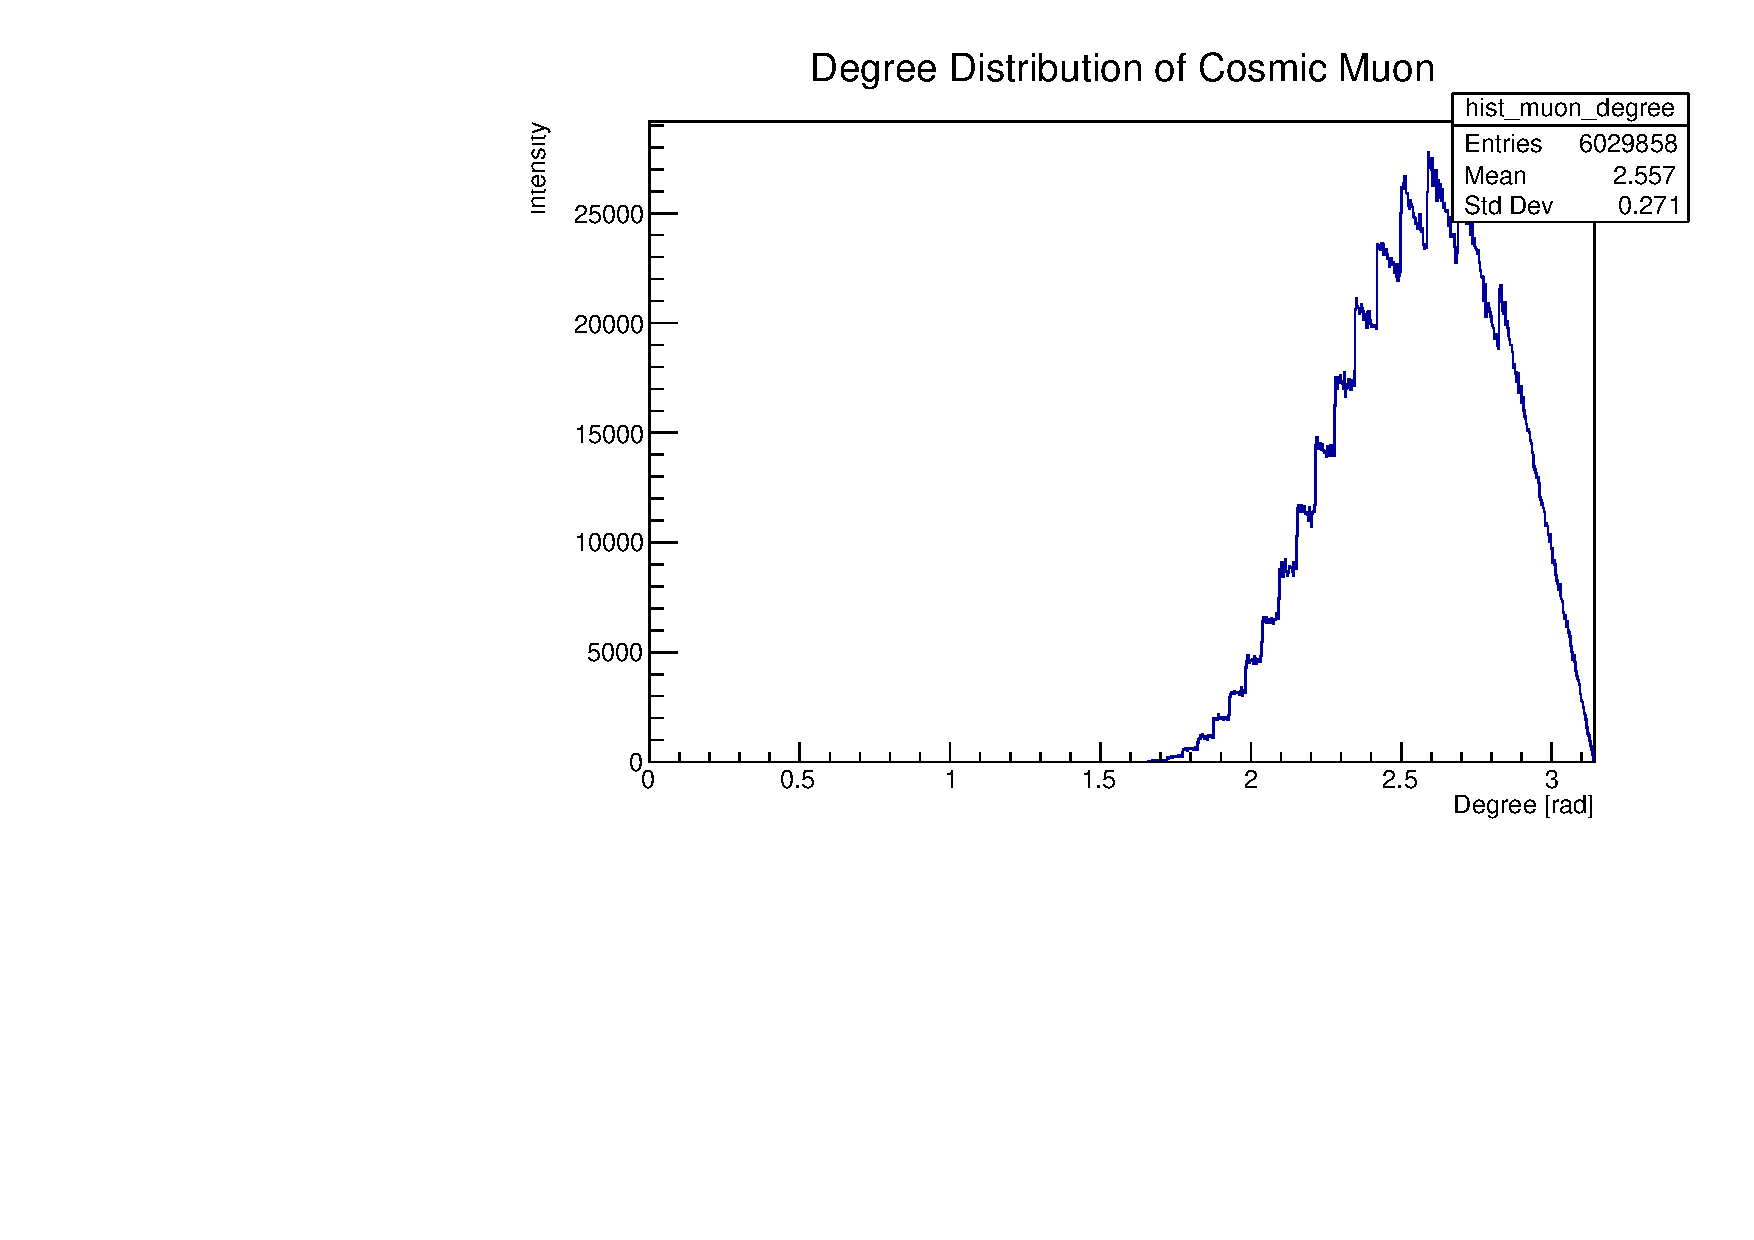
\includegraphics[height=5cm]{img/muon_degree_distribution.pdf}
        \caption{CRYによって生成した$\mu$粒子の角度分布}
        \label{fig:muon_degree_distribution}
    \end{minipage}
\end{figure}
図\ref{fig:muon_energy_distribution}より、入射$\mu$粒子は2000MeVあたりのエネルギーを持ったものが多いがそれよりも高エネルギーな粒子も存在するということがわかる。
図\ref{fig:muon_degree_distribution}においてdegree 0 は$z$軸正の方向を指しているので分布より斜め下向きに入射している粒子が多いことがわかる。
また、ヒストグラムのエントリー数が約600万イベントであることよりトリガーシンチレータを通過してもすべての粒子が検出器に入射するわけではないということがわかる。

今回シミュレーションを行った目的としては, 検出器内での光生成反応がどれくらいの割合で発生するのか求めることである.

\section{シミュレーション結果}
今回のシミュレーションにおいては光生成反応として入射$\mu$粒子からパイオンが発生したイベントを選んだ.

一番下のシンチレータまで$\mu$粒子が到達したイベントは全イベントのうち1,937,095イベントで効率は0.194であった.
また, シンチレータ内で反応して$\pi$が出たイベントは19イベントで効率は$1.90 \times10^{-6}$であった.
実際の測定器に$\mu$粒子が入射するレートは15count/secであったので, 1秒に$2.85 \times10^{-5}$だけ$\pi$が出てくるイベントがあるということになる.
実際約260時間測定を行ったので$1.2 \times10^{7}$万イベント得られた.
このことより, 今回用いた検出器においても光生成反応が起きて$\pi$が出てくるイベントというのが数十イベントくらいは観測できそうだということがわかった.

\begin{table}[H]
    \centering
    \caption{シミュレーションによるデータ}
    \label{tab:simu_data}
    \begin{tabular}{|c|r|}
        \hline
        総イベント                               & 10,000,000 \\ \hline
        1番下の層まで$\mu$粒子が通過したイベント & 1,937,095  \\ \hline
        $\pi$が出たイベント                      & 19         \\ \hline
    \end{tabular}
\end{table}

下の図\ref{fig:simu_track},\ref{fig:simu_pixel}は, 後述(\ref{sec:anal:eventcut}節)する解析プログラムを用いてシミュレーションデータを解析した図である.
このイベントだと宇宙線$\mu$粒子が検出器内で反応して2粒子出たことがわかる.それぞれの粒子の失ったエネルギーをシミュレーション結果から計算するとどの粒子か特定することができる。
\begin{figure}[H]
    \begin{minipage}[b]{0.47\linewidth}
        \centering
        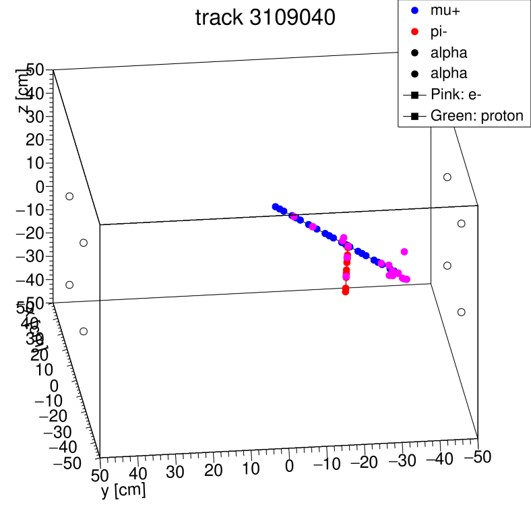
\includegraphics[height=5cm]{img/track_pion.jpg}
        \caption{検出器内でのトラックの様子}
        \label{fig:simu_track}
    \end{minipage}[b]
    \begin{minipage}[b]{0.47\linewidth}
        \centering
        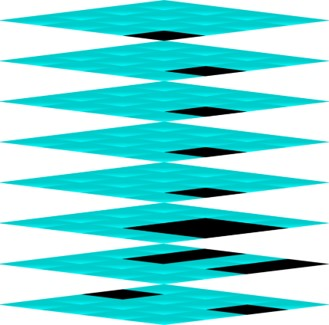
\includegraphics[height=5cm]{img/track_simulation.jpg}
        \caption{各シンチレータの鳴ったピクセル}
        \label{fig:simu_pixel}
    \end{minipage}
\end{figure}


\chapter{実験の準備}\label{preparation}
\section{予備実験}

\chapter{解析}\label{analysis}
測定データを用いてどのように光生成反応イベントを探索したかを説明する。

\section{解析に用いたデータ}\label{sec:anal:data}
表\ref{tab:analyzed_data}に示すようにトリガーレート15\ cps, データ取得時間約260時間, 取得イベント数12054470イベントのデータを解析に用いた.
\begin{table}[H]
    \centering
    \caption{解析に用いたデータ}
    \label{tab:analyzed_data}
    \begin{tabular}{|c|r|}
        \hline
        トリガーレート & 15 cps    \\ \hline
        取得時間       & 約260時間 \\ \hline
        イベント数     & 12054470  \\ \hline
    \end{tabular}
\end{table}

\section{しきい値の設定}\label{sec:anal:threshold}
\ref{sec:mppc_gain_diff}節の通り、ADC value は荷電粒子がシンチレータに渡したエネルギーに比例している量であるのでADC valueに適切なしきい値を設けることでシンチレータ毎に荷電粒子が通過したかどうかを判別できる.
シンチレータがエネルギーを受け取らなかった時のADC value は本実験で用いたEASIROCにおいては典型的に800付近であったため(図\ref{fig:mu_mppc}, \ref{fig:threhist}), ADC value 800付近からある程度離れた値をしきい値とすることにした.
具体的には図\ref{fig:adc_eff}のようにADC value のしきい値を800から1500まで1刻みで変更した時の検出効率を計算し, チャンネル毎にeffeciencyが大きく下がらない程度のしきい値を探すことでしきい値を決定した.
図\ref{fig:adc_eff}, \ref{fig:threhist} の赤線は実験に用いたADC valueのしきい値を示している。
\begin{figure}[H]
    \centering
    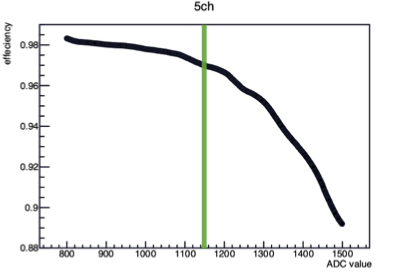
\includegraphics[height=5.0cm]{img/adc_eff.png}
    \caption{しきい値と検出効率の関係}
    \label{fig:adc_eff}
\end{figure}
\begin{figure}[H]
    \centering
    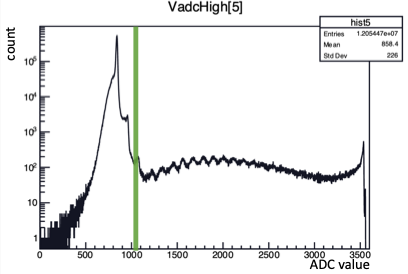
\includegraphics[height=5.0cm]{img/pedestal.png}
    \caption{宇宙線による ADC value の分布}
    \label{fig:threhist}
\end{figure}

\section{ヒット情報の作成}
\subsection{ヒット情報の作成方法}\label{subsec:anal:make_hit}
\ref{sec:anal:threshold} 節で荷電粒子が64枚あるシンチレータのうちのどのシンチレータを通過したかという情報を得ることができた.図\ref{fig:igata01}は実験装置のある層でシンチレータに荷電粒子が走ったか/走っていなかったかを色分けしたものである.図の赤く塗られている部分のように, 荷電粒子はしきい値を超えたシンチレータ同士が重なる位置を通過したと考えることができる.図\ref{fig:igata01}は1層分の絵であるが, 8層分に以上の処理を施すことでで荷電粒子の3次元飛跡のようなものの情報が得られた(図\ref{fig:eventdisplay}).図\ref{fig:eventdisplay}の透過している青い領域は検出器の有感領域を示しており、黒い領域は解析によって荷電粒子がと通過したと判定された領域である。この3次元飛跡のようなものから飛跡を再構成することができる.
\begin{figure}[H]
    \begin{tabular}{cc}
        \begin{minipage}[t]{0.45\hsize}
            \centering
            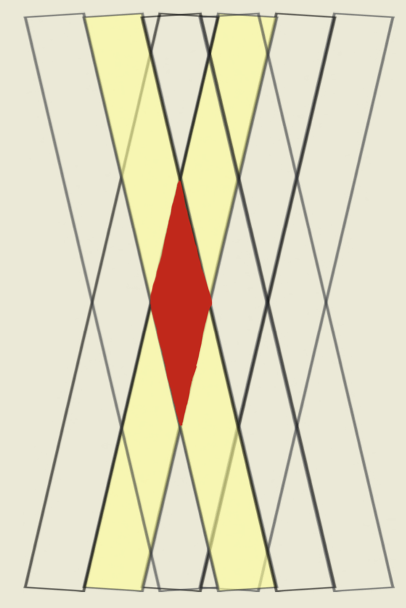
\includegraphics[height=5.0cm]{img/igata_01.png}
            \caption{1層分のシンチレータ}
            \label{fig:igata01}
        \end{minipage}
        \begin{minipage}[t]{0.45\hsize}
            \centering
            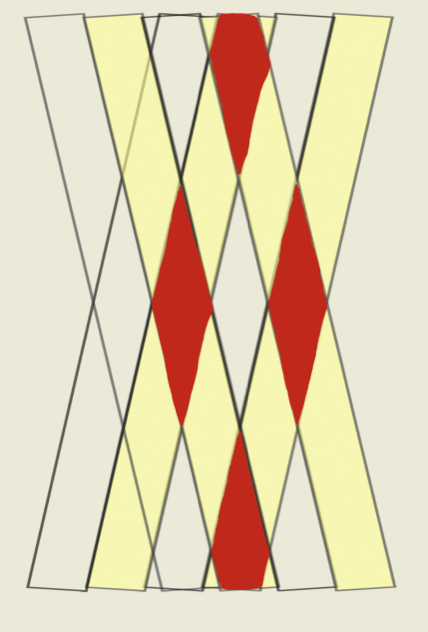
\includegraphics[height=5.0cm]{img/igata_02.png}
            \caption{1層に2つ以上の荷電粒子が通ったとき}
            \label{fig:igata02}
        \end{minipage}
    \end{tabular}
\end{figure}
\begin{figure}[H]
    \centering
    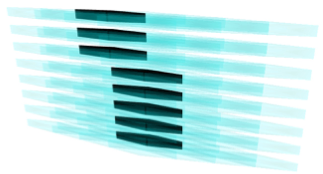
\includegraphics[height=5.0cm]{img/eventdisplay.png}
    \caption{イベントディスプレイ}
    \label{fig:eventdisplay}
\end{figure}
\subsection{ヒット情報作成の問題点}
\ref{subsec:anal:make_hit}節で説明したヒット情報の計算方法には問題点が存在する.
1層に2個以上の荷電粒子が通過した場合に作成されたヒット情報からは飛跡を再構成できないという点である.
例えば, 図\ref{fig:igata02}に示すようにシンチレータから得られたADC valueがしきい値を超えた場合は赤く塗られる箇所(荷電粒子が通過したと考えられる場所)が余分にできてしまい, 荷電粒子の本当の飛跡がわからなくなってしまう.本実験では光生成反応を探索しているため探索対象は複数の粒子の飛跡であるが, この問題点は複数の粒子の飛跡の再構成を難しくしてしまっている.

\section{光生成反応イベントの探索}
\subsection{イベントセレクション}\label{sec:anal:eventcut}
\ref{sec:anal:data}に示した測定データから光生成反応と考えられるイベントを以下に示す条件によってカットをかけた.
\begin{itemize}
    \item[(1)] 6層以上の層を荷電粒子が通った
    \item[(2)] 1, 2, 8層目で1つの荷電粒子が通った
    \item[(3)] 3〜7層目で荷電粒子の反応が2つ以上ある
\end{itemize}
(1), (2)の条件は荷電粒子が検出器内をある程度真っ直ぐ通ったことを保証するための条件である.(3)の条件は光生成反応によって期待される複数粒子の飛跡を捉えるための条件である.

イベントセレクションの結果残ったイベントは2543イベントであり, 総取得イベント数12054473の約0.021\%であった.イベントセレクションによって得られたイベントの例を図\ref{fig:eventcuted_event}に示す.図\ref{fig:eventcuted_event}は上から順にz軸正の方向から各層を示していて, 一つの菱形がピクセルを表しており, 黒く塗りつぶされたピクセルが荷電粒子が検出器を通ったと考えられるピクセルである.図\ref{fig:eventcuted_event}を見ると, ミューオンがz軸正の方向から検出器に入射し, 3層目あたりでもう一つの荷電粒子が発生したと見ることができる.しかし, このイベントが光生成反応によって得られたイベントであるかどうかは定かではない.
\begin{figure}[H]
    \centering
    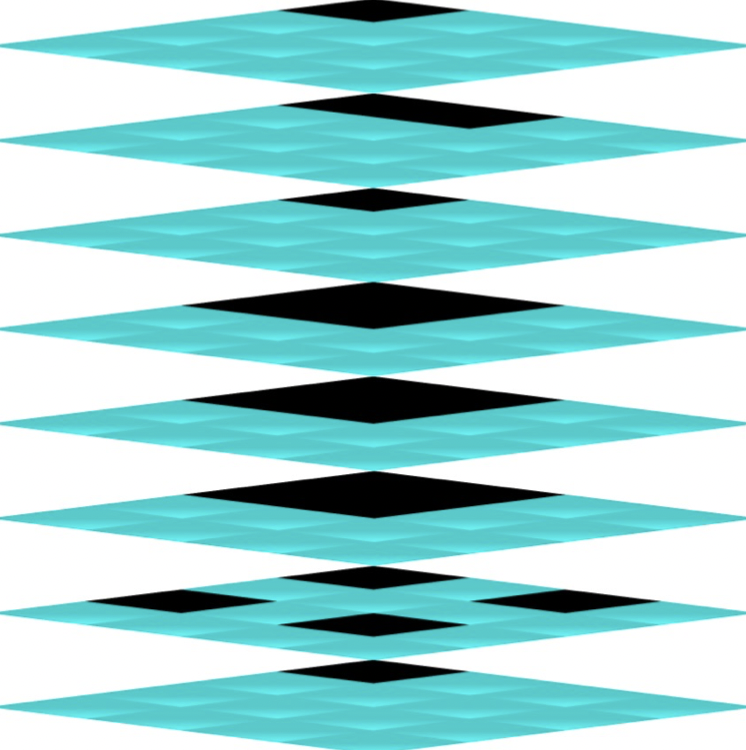
\includegraphics[height=5.0cm]{img/eventcutted_figure.png}
    \caption{イベントセレクション後のイベントの例}
    \label{fig:eventcuted_event}
\end{figure}

\subsection{イベントセレクションの検証}\label{sec:eventcut_val}
\ref{sec:anal:eventcut}節のイベントセレクションによって得られたイベントは光生成反応由来かどうか定かではないと述べた.そこで, シミュレーションによって得られたデータを\ref{sec:anal:eventcut}節と同じイベントセレクションで解析することによってイベントセレクションによってどれだけの光生成反応イベントが得られたかどうかを検証した.結果を表\ref{tab:eventcut_val}に示す.
\begin{table}[H]
    \centering
    \caption{イベントセレクションの検証}
    \label{tab:eventcut_val}
    \begin{tabular}{|c|c|}
        \hline
        \begin{tabular}[c]{@{}c@{}}全イベント\\ 10000000\end{tabular}                     & \begin{tabular}[c]{@{}c@{}}カット後\\ 5759\end{tabular}                       \\ \hline
        \begin{tabular}[c]{@{}c@{}}全イベント中でパイオンを含むイベント\\ 19\end{tabular} & \begin{tabular}[c]{@{}c@{}}カット後でパイオンを含むイベント\\ 14\end{tabular} \\ \hline
    \end{tabular}
\end{table}
表\ref{tab:eventcut_val}によるとイベントセレクション前とイベントセレクション前でパイオンイベントの純粋度は0.00019\%から0.24\%に上昇していることがわかる.しかし, カット後のイベントにおけるパイオンイベントの純粋度が0.24\%というのはイベントセレクションでは取り除けなかったバックグラウンドの存在が示唆される.よって, \ref{sec:anal:eventcut}節で行ったイベントセレクションではバックグラインドが十分に取り除くことができなかったといえる.

\subsection{バックグラウンドの検討}\label{sec:anal:background}
図\ref{fig:anal:bg01}は\ref{sec:eventcut_val}節で使用したシミュレーションデータから, イベントセレクションがパイオンイベントと間違えたイベントを可視化したものの例である.図\ref{fig:anal:bg01}に示すようなミューオンが検出器内の電子を弾くイベントが支配的であった。図\ref{fig:pion_electron_degrere}はシミュレーションによって得られた, ミューオンによって弾き出された電子とパイオンの角度分布である。青色、赤色で表されるヒストグラムはそれぞれ光生成反応によって生成されたパイオン、ミューオンによって蹴り出された電子の散乱角分布を示している。角度は上空方向を正としたベクトル(図\ref{fig:arrangement}におけるz軸)と粒子の運動量ベクトルの内積によって定義される。本研究において用いたイベントセレクションでは主に、入射ミューオンと同じ方向へ飛ぶパイオンを検出しようとしたために図\ref{fig:pion_electron_degrere}における$\pi$ラジアン付近の探索をしていた。そのために電子散乱におけるイベントがイベントセレクション後のイベントに含まれていたと考えられる。
\begin{figure}[H]
    \centering
    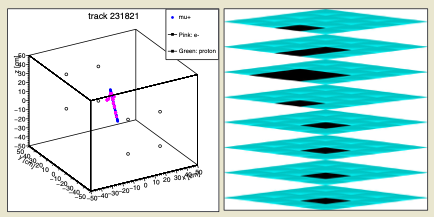
\includegraphics[height=5.0cm]{img/anal_bg01.png}
    \caption{バックグラウンドと考えられるイベント}
    \label{fig:anal:bg01}
\end{figure}
\begin{figure}[H]
    \centering
    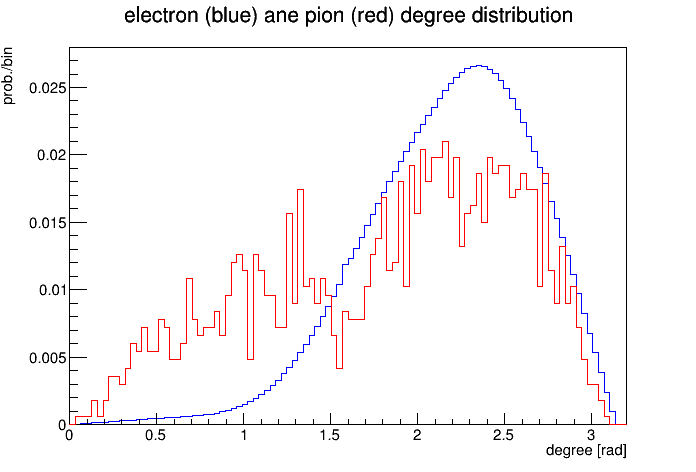
\includegraphics[height=5.0cm]{img/pi_e_degree.png}
    \caption{パイオンと電子の角度分布}
    \label{fig:pion_electron_degrere}
\end{figure}
\chapter{結論}\label{cha:conclusion}
本研究の目的は光生成反応の飛跡を捉えることが目的であったが, うまく捉えることができなかった.
以下に示す2点の改良及び解析で光生成反応の飛跡を捉えることができるであろうと考えられる.

1つ目は装置のデザインの見直しである.本研究では納期や予算の都合上新しいシンチレータを用いることが難しい状況にあり, 既存のシンチレータを用いて光生成反応の検出に取り組む必要があった.その結果として棒状の長いシンチレータを斜めに交差させることで3次元飛跡検出器を作ることになった.この検出器は光生成反応を探索するには横方向の位置分解能が低いという問題点があるため, 横方向の位置分解能が良い検出器をデザインし直すことで光生成反応イベントの探索が容易になるであろうと考えられる.

2つ目はバックグラウンドの低減を図ることである.例えば、\ref{sec:anal:background}節で述べたようなパイオンと電子の角度分布の違いを利用して、実験装置と解析の両方において光生成反応によって生成されたパイオンが支配的な角度範囲に感度を持たせることなどが挙げられる。
\chapter{謝辞}\label{acknowledgements}


\printbibliography[title = 参考文献]

\end{document}